\documentclass[12pt]{article}
\usepackage[T1]{fontenc}
\usepackage{enumitem}
\usepackage[english]{babel}
\usepackage{graphicx,epstopdf,url}
\usepackage{float}
\usepackage{amsmath}
\usepackage{booktabs}

\usepackage[top=0.8in, bottom=1in, left=1in, right=1in]{geometry}

\title{Performance Evaluation - Lab report \\

Discrete Event Simulator for Queueing Systems
}
\author{\bf{Group 10} \\ \\
        Abdul Hadi Farooq \\
        Ali Haider \\
        Ali Raza \\
}

\date{May 7, 2026}

\begin{document}

\maketitle

\section{Introduction}

The objective of this lab is to understand performance evaluation of computer systems through discrete-event simulation of queueing models. We implemented a discrete-event simulator using an object-oriented design that models message-based systems with queueing and service components. The simulator handles four queueing scenarios: M/M/1, M/M/1/4, M/M/1/8, and M/M/3/8.

Queueing theory is useful for understanding computer systems, communication networks, and data centers, where randomness is present in both arrival and service processes. By simulating these systems under different load conditions, we can estimate performance metrics and understand system behavior before actual deployment.

This laboratory explores four classic queueing scenarios:
\begin{itemize}
    \item \textbf{M/M/1:} Single server, infinite capacity queue
    \item \textbf{M/M/1/4:} Single server, maximum 4 entities in system (capacity-limited)
    \item \textbf{M/M/1/8:} Single server, maximum 8 entities in system (capacity-limited)
    \item \textbf{M/M/3/8:} Three parallel servers, maximum 8 entities in system
\end{itemize}

For each model, we evaluate performance across varying arrival rates $\lambda \in \{4, 6, 8, 12\}$ messages per second, with fixed service rate $\mu = 8$ messages per second. Performance metrics include average system occupancy, queue length, waiting time, throughput, server utilization, and loss probability for capacity-limited systems.

\subsection{Methodology}

\begin{itemize}
    \item \textbf{Programming Language:} Python 3.14 with NumPy (random generation) and Matplotlib (plotting)
    \item \textbf{Simulator Architecture:} Object-oriented design with Message, Event, Scheduler, Client, Queue, Server, and Gateway classes
    \item \textbf{Simulation Parameters:}
          \begin{itemize}
              \item Simulation time per run: 5,000 seconds
              \item Warmup period: 500 seconds (10\% of simulation time)
              \item Independent replications: 100 runs per configuration
              \item Total configurations: 16 (4 scenarios $\times$ 4 arrival rates)
              \item Total replication runs: 1600
          \end{itemize}
    \item \textbf{Statistical Analysis:} 95\% confidence intervals computed via the t-distribution
    \item \textbf{Reproducibility:} Deterministic seeding based on scenario and replication index ensures reproducible results
    \item \textbf{Event Model:}
          \begin{itemize}
              \item SEND\_MSG: Client sends message (source=client, destination=gateway)
              \item RECV\_MSG: Gateway receives message (after 1-second propagation delay)
              \item MSG\_DEPT: Service completion at gateway and message departure from system
          \end{itemize}
\end{itemize}

\subsection{Code Repository}

Our implementation is available at:

\begin{center}
    \url{https://github.com/abdulhadihub/cnam-performance-evaluation-course/tree/main/lab-2}
\end{center}

The project includes the following modules:
\begin{itemize}
    \item \texttt{sim/message.py} - Message class
    \item \texttt{sim/event.py} - Event class and EventType enum
    \item \texttt{sim/scheduler.py} - Min-heap event scheduler
    \item \texttt{sim/client.py} - Client generating exponential inter-arrival times
    \item \texttt{sim/queue\_model.py} - FIFO queue
    \item \texttt{sim/server.py} - Server with exponential service times
    \item \texttt{sim/gateway.py} - Gateway orchestrating queue and server pool
    \item \texttt{sim/engine.py} - Main event loop and metrics collection
    \item \texttt{sim/experiments.py} - Batch runner and plotting
    \item \texttt{main.py} - CLI entry point
\end{itemize}

\section{System Architecture}

\subsection{Design Overview}

The simulator works as follows:

\begin{enumerate}
    \item \textbf{Scheduler:} Maintains events in chronological order. Uses a min-heap to achieve O(log n) insertion without full re-sorting.
    \item \textbf{Event Loop:} Repeatedly extracts the earliest event, updates system state, and may schedule new events.
    \item \textbf{Components:} Each system component (Client, Queue, Server, Gateway) is modeled as an object with state and methods.
    \item \textbf{Message Tracking:} Messages carry metadata (ID, source, destination, creation time) to compute response times and queue waits.
    \item \textbf{Metrics Collection:} After each event, system state is recorded for time-weighted and count-based metric computation.
    \item \textbf{Trace Generation:} A CSV trace file records every event (time, node, event type, source, destination, message ID).
\end{enumerate}

\subsection{Queueing Model Details}

\subsubsection{Capacity Convention}

In our M/M/1/K models, the capacity $K$ is the total number of entities allowed in the system at any time (including both the one in service and those waiting in queue):
\begin{itemize}
    \item M/M/1: No capacity limit
    \item M/M/1/4: Maximum 4 entities total (if all 4 are occupied, new arrivals are dropped)
    \item M/M/1/8: Maximum 8 entities total
    \item M/M/3/8: Maximum 8 entities with 3 parallel servers
\end{itemize}

\subsubsection{Arrival Process}

Inter-arrival times follow an exponential distribution with mean $1/\lambda$:
\begin{equation}
    \text{Inter-arrival time} \sim \text{Exponential}(\lambda)
\end{equation}

For example, with $\lambda = 6$ messages/s, the mean inter-arrival time is $1/6 \approx 0.167$ seconds.

\subsubsection{Service Process}

Service times follow an exponential distribution with mean $1/\mu = 1/8 = 0.125$ seconds:
\begin{equation}
    \text{Service time} \sim \text{Exponential}(\mu)
\end{equation}

All servers in all scenarios have the same $\mu = 8$ messages/s, so M/M/3 systems have aggregate service capacity of $3 \times 8 = 24$ messages/s when all three servers are busy.

\subsubsection{Queue Discipline}

All queues follow FIFO (First-In-First-Out) discipline. When a server becomes idle:
\begin{itemize}
    \item If queue is not empty: next message from queue begins service immediately
    \item If queue is empty: server becomes idle, waiting for next arrival
\end{itemize}

For capacity-limited systems, if the system is full when an arrival occurs, that message is dropped and not served.

\section{Metrics}

\subsection{Time-Weighted Metrics}

After warmup period, the simulator computes:

\begin{enumerate}
    \item \textbf{Average System Occupancy:} Mean number of entities in system (queue + in service)
          \begin{equation}
              N_s = \frac{1}{T} \int_0^T N(t) \, dt
          \end{equation}
          where $N(t)$ is the instantaneous system occupancy and $T$ is the measured time interval after warmup.

    \item \textbf{Average Queue Length:} Mean number of entities waiting in queue (not in service)
          \begin{equation}
              N_q = \frac{1}{T} \int_0^T N_q(t) \, dt
          \end{equation}

    \item \textbf{Average Server Utilization:} Per-server utilization (fraction of time each server is busy, averaged across all servers)
          \begin{equation}
              \rho = \frac{\text{Total server busy time}}{T \times \text{Number of servers}}
          \end{equation}
\end{enumerate}

\subsection{Count-Based Metrics}

\begin{enumerate}
    \item \textbf{Throughput:} Number of completed messages per unit time (after warmup)
          \begin{equation}
              \text{Throughput} = \frac{\text{Departures after warmup}}{T}
          \end{equation}

    \item \textbf{Average Queue Waiting Time:} Mean time spent waiting in queue before service
          \begin{equation}
              W_q = \frac{\sum \text{Wait times}}{N_{\text{departures}}}
          \end{equation}

    \item \textbf{Average Response Time:} Mean time from arrival to departure (total time in gateway, queue + service)
          \begin{equation}
              W = \frac{\sum (\text{Departure time} - \text{Arrival time})}{N_{\text{departures}}}
          \end{equation}

    \item \textbf{Average Service Time:} Mean time spent in the servers (response time minus queue wait)
          \begin{equation}
              W_{\text{svr}} = W - W_q
          \end{equation}

    \item \textbf{Drop Probability (capacity-limited systems):} Fraction of arrivals that are dropped
          \begin{equation}
              P_{\text{drop}} = \frac{\text{Dropped arrivals}}{\text{Total arrivals}}
          \end{equation}
\end{enumerate}

\subsection{Confidence Intervals}

For each metric and configuration, we compute a two-sided 95\% confidence interval using the t-distribution:

\begin{equation}
    \text{CI} = \bar{x} \pm t_{0.975}(n-1) \cdot \frac{s}{\sqrt{n}}
\end{equation}

where:
\begin{itemize}
    \item $\bar{x}$ is the sample mean across 100 replications
    \item $s$ is the sample standard deviation
    \item $t_{0.975}(n-1)$ is the two-sided t critical value (for $n > 30$, the normal approximation $z_{0.975} \approx 1.96$ is used)
    \item $n = 100$ is the number of replications
\end{itemize}

\section{Results}

\subsection{M/M/1: Unlimited Capacity, Single Server}

\subsubsection{Theoretical Background}

The M/M/1 queue has well-known analytical results when the system is stable ($\rho = \lambda/\mu < 1$):

\begin{itemize}
    \item Average system occupancy: $N_s = \frac{\rho}{1 - \rho}$
    \item Average queue length: $N_q = \frac{\rho^2}{1 - \rho}$
    \item Average wait in queue: $W_q = \frac{\rho}{\mu(1-\rho)}$
    \item Average response time: $W = \frac{1}{\mu(1-\rho)}$
    \item Utilization: $\rho = \lambda/\mu$
    \item Stability condition: $\rho < 1$ (i.e., $\lambda < \mu$)
\end{itemize}

For our scenario with $\mu = 8$:
\begin{itemize}
    \item $\lambda = 4$: $\rho = 0.5$, stable
    \item $\lambda = 6$: $\rho = 0.75$, stable
    \item $\lambda = 8$: $\rho = 1.0$, marginally unstable (infinite queue at equilibrium)
    \item $\lambda = 12$: $\rho = 1.5$, unstable (queue grows without bound)
\end{itemize}

\subsubsection{Average System Occupancy}

\begin{figure}[H]
    \centering
    
\includegraphics[width=0.75\textwidth]{../outputs/plots/MM1-avg_n_system.png}
    \caption{M/M/1: Average system occupancy vs. arrival rate. With 95\% CI error bars.}
    \label{fig:mm1-n_system}
\end{figure}

\subsubsection{Average Messages in Queue}

\begin{figure}[H]
    \centering
    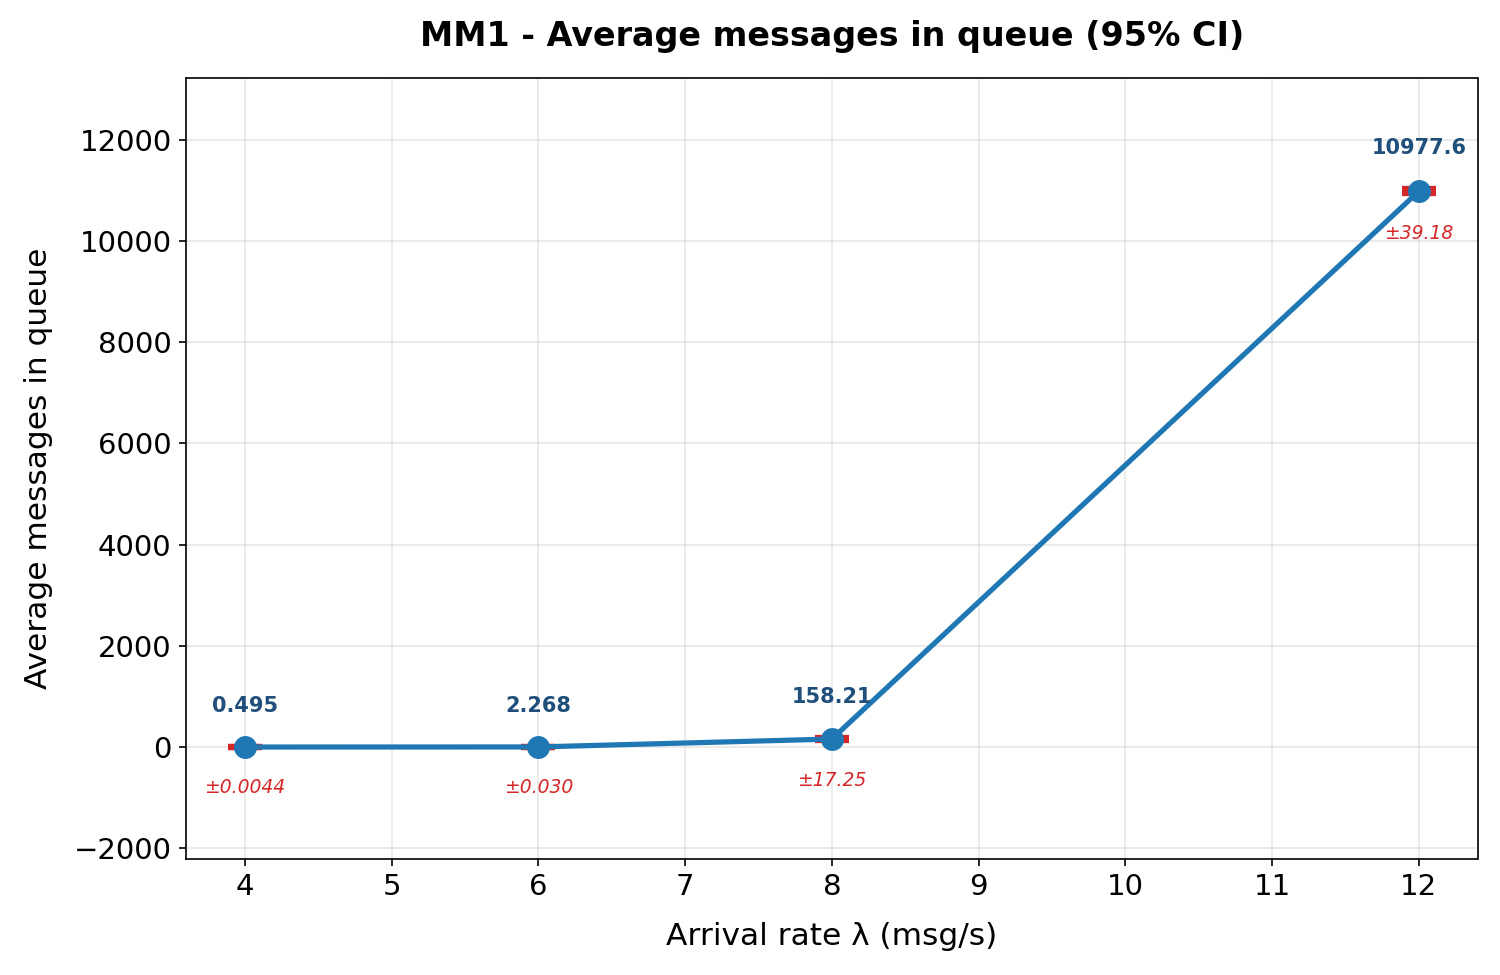
\includegraphics[width=0.75\textwidth]{../outputs/plots/MM1-avg_n_queue.png}
    \caption{M/M/1: Average number of messages in queue vs. arrival rate. With 95\% CI error bars.}
    \label{fig:mm1-n_queue}
\end{figure}

\subsubsection{Average Queue Waiting Time}

\begin{figure}[H]
    \centering
    
\includegraphics[width=0.75\textwidth]{../outputs/plots/MM1-avg_wait_queue.png}
    \caption{M/M/1: Average queue wait time vs. arrival rate. With 95\% CI error bars.}
    \label{fig:mm1-wait_queue}
\end{figure}

\subsubsection{Average Time in the Gateway}

\begin{figure}[H]
    \centering
    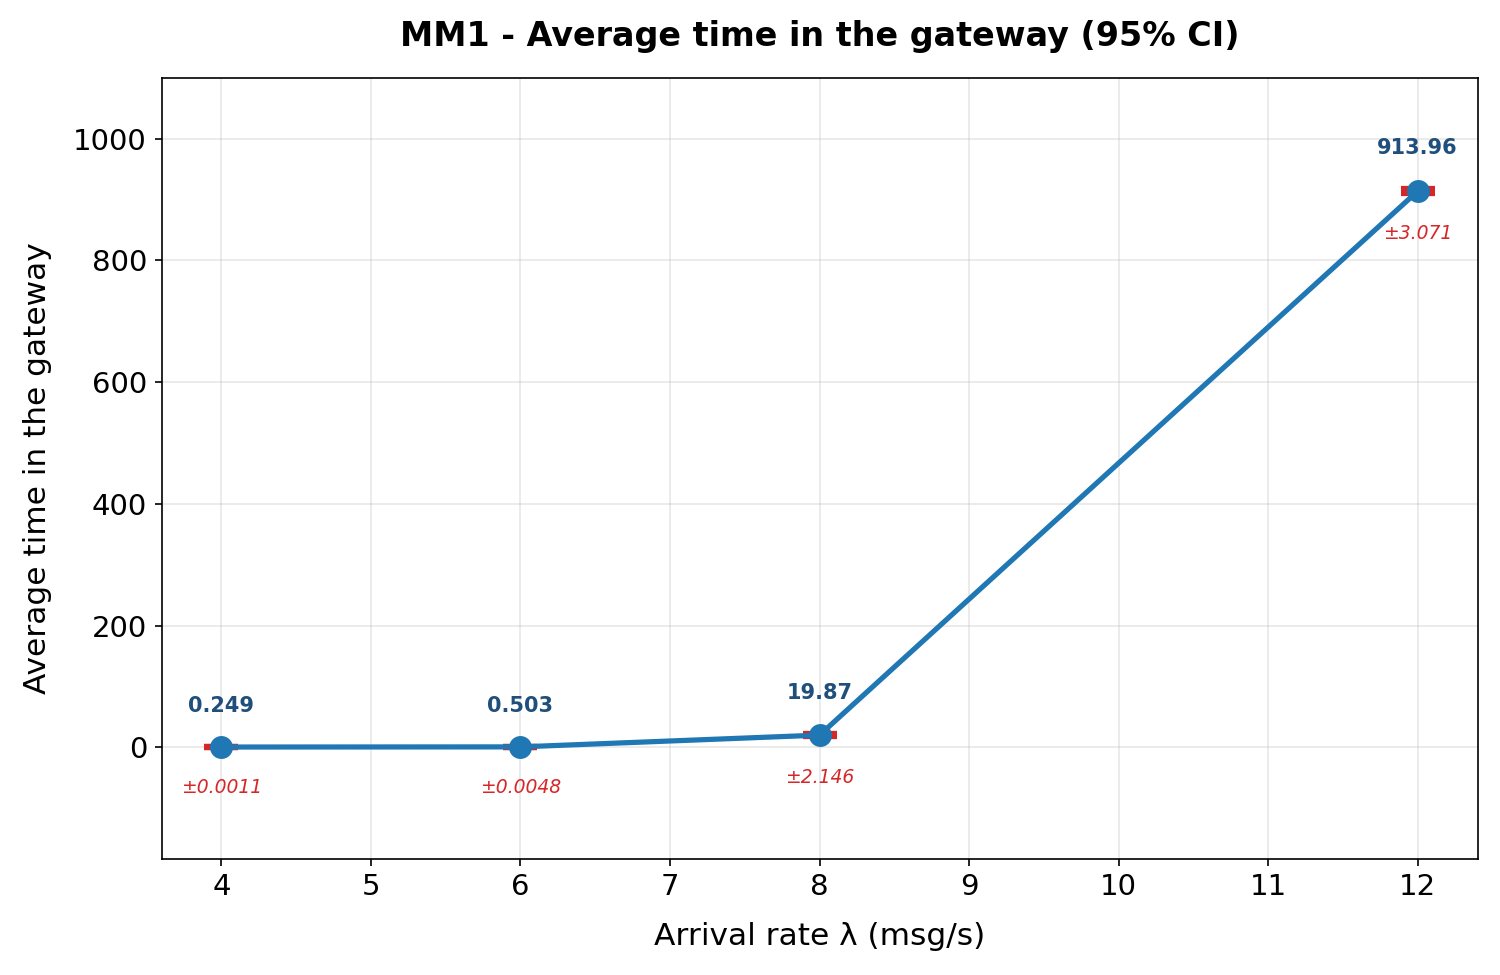
\includegraphics[width=0.75\textwidth]{../outputs/plots/MM1-avg_response_time.png}
    \caption{M/M/1: Average time in the gateway vs. arrival rate. With 95\% CI error bars.}
    \label{fig:mm1-response_time}
\end{figure}

\subsubsection{Average Time in the Servers}

\begin{figure}[H]
    \centering
    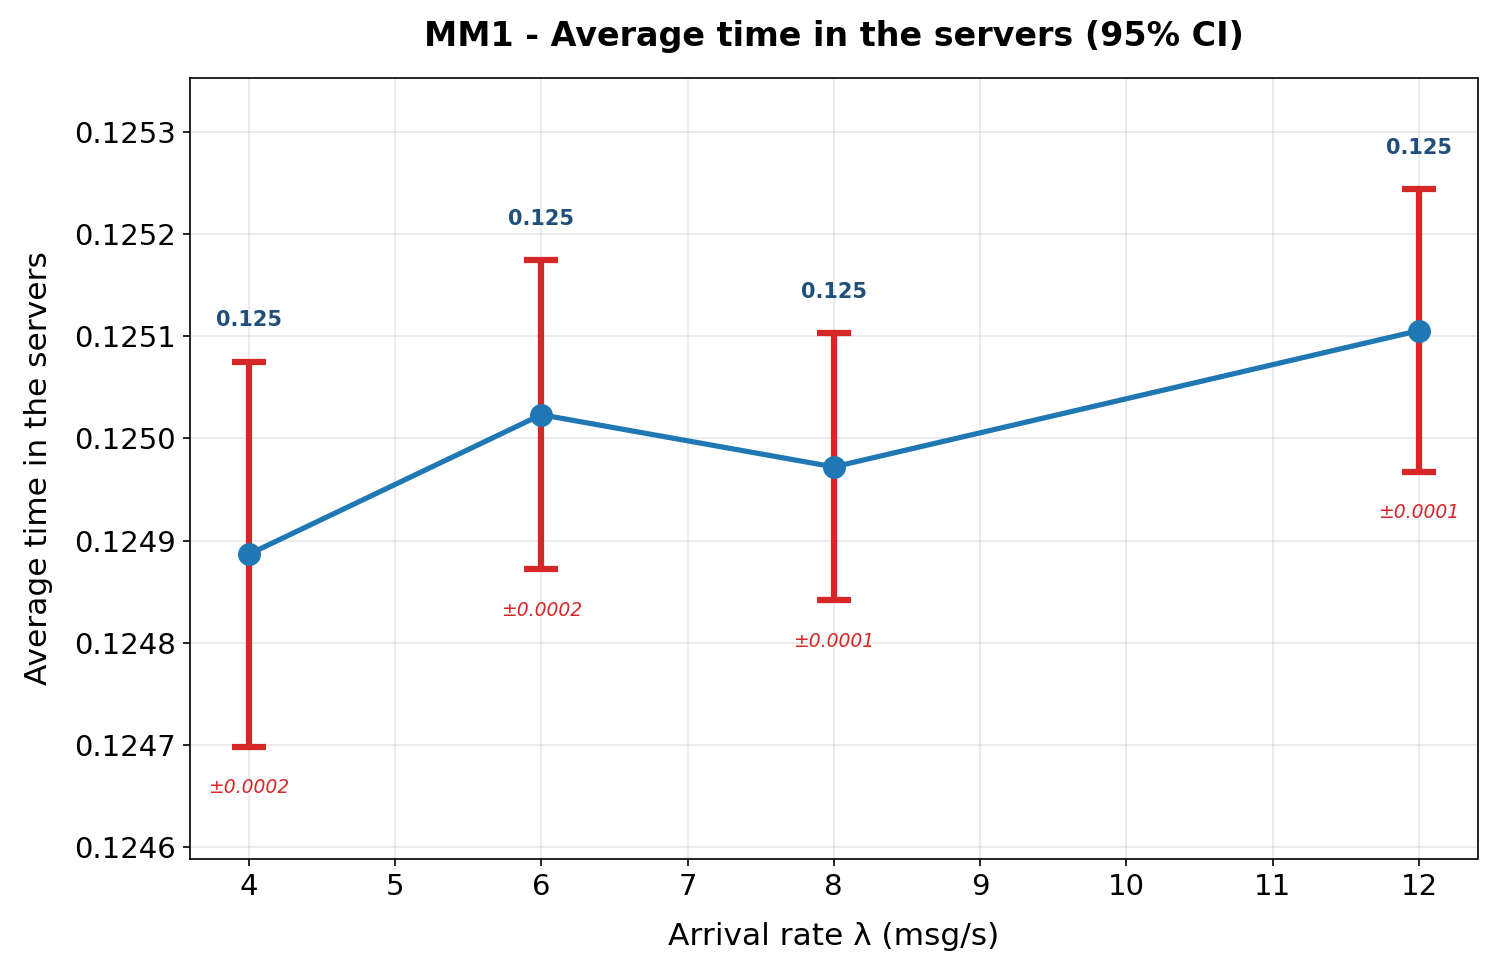
\includegraphics[width=0.75\textwidth]{../outputs/plots/MM1-avg_time_in_servers.png}
    \caption{M/M/1: Average time in the servers vs. arrival rate. With 95\% CI error bars.}
    \label{fig:mm1-time_in_servers}
\end{figure}

\subsubsection{Throughput}

\begin{figure}[H]
    \centering
    
\includegraphics[width=0.75\textwidth]{../outputs/plots/MM1-throughput.png}
    \caption{M/M/1: Throughput vs. arrival rate. With 95\% CI error bars.}
    \label{fig:mm1-throughput}
\end{figure}

\subsubsection{Drop Probability}

\begin{figure}[H]
    \centering
    
\includegraphics[width=0.75\textwidth]{../outputs/plots/MM1-drop_probability.png}
    \caption{M/M/1: Drop probability vs. arrival rate. With 95\% CI error bars. (Always zero for unlimited capacity.)}
    \label{fig:mm1-drop}
\end{figure}

\subsubsection{Observations}

For the M/M/1 queue:

\begin{itemize}
    \item \textbf{$\lambda = 4$ (low load):} System remains lightly loaded with $\rho = 0.5$. Average occupancy is about 1 entity, and queue waits are minimal ($\sim 0.12$ seconds). Throughput matches arrival rate closely.

    \item \textbf{$\lambda = 6$ (moderate load):} System is moderately loaded with $\rho = 0.75$. Average occupancy rises to $\sim 3$ entities, and queue wait becomes noticeable ($\sim 0.38$ seconds). Throughput remains close to arrival rate.

    \item \textbf{$\lambda = 8$ (saturation):} System reaches saturation ($\rho = 1.0$). Queue grows quickly, and both occupancy and wait times increase significantly. Throughput saturates around $\mu = 8$ messages/s.

    \item \textbf{$\lambda = 12$ (overload):} System is unstable ($\rho = 1.5$). Queue grows without bound over the simulation horizon. Measured metrics reflect the transient behavior before queue saturation; in reality, such conditions require admission control.

    \item \textbf{Confidence Intervals:} At lower loads ($\lambda \le 6$), CI widths are narrow, indicating stable, reproducible behavior. At higher loads, CI widens, reflecting increased variability in queue dynamics.
\end{itemize}

\subsection{M/M/1/4: Single Server with Capacity 4}

\subsubsection{Theoretical Background}

For M/M/1/K, the system has a maximum capacity $K$. New arrivals when the system is full are lost. Theoretical steady-state results:

\begin{itemize}
    \item If $\rho \ne 1$: $P_n = (1-\rho) \rho^n / (1 - \rho^{K+1})$ for $n = 0, 1, \ldots, K$
    \item Loss probability: $P_K = (1-\rho) \rho^K / (1 - \rho^{K+1})$
    \item Effective arrival rate: $\lambda_{\text{eff}} = \lambda(1 - P_K)$
\end{itemize}

With capacity 4 and $\mu = 8$, the system blocks when 4 entities are present.

\subsubsection{Average System Occupancy}

\begin{figure}[H]
    \centering
    
\includegraphics[width=0.75\textwidth]{../outputs/plots/MM1K4-avg_n_system.png}
    \caption{M/M/1/4: Average system occupancy vs. arrival rate. With 95\% CI error bars.}
    \label{fig:mm1k4-n_system}
\end{figure}

\subsubsection{Average Messages in Queue}

\begin{figure}[H]
    \centering
    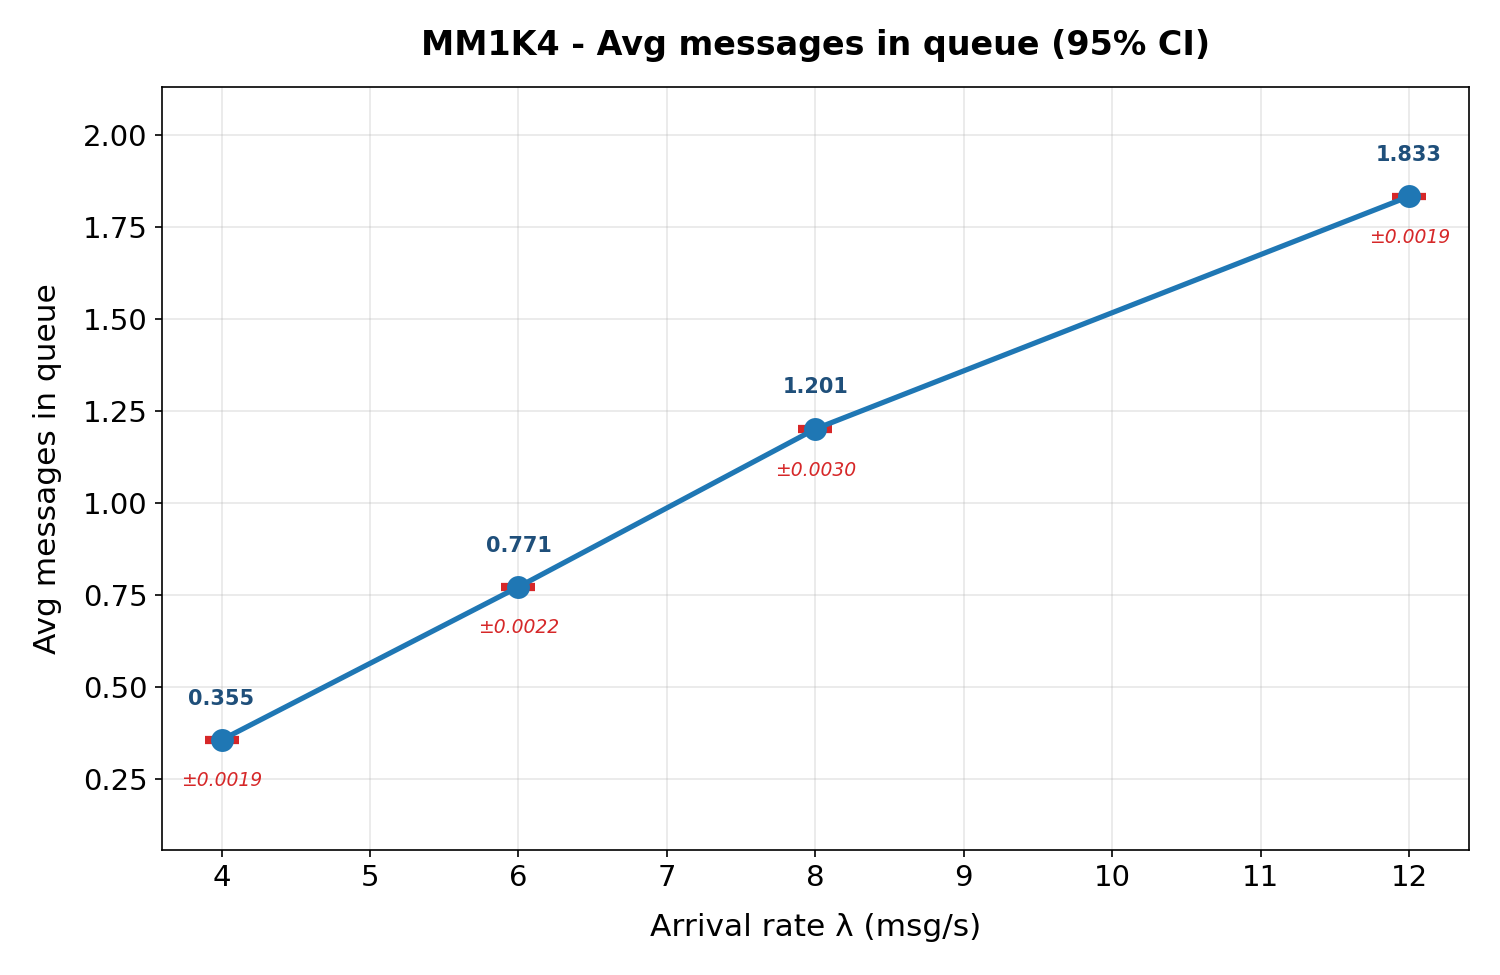
\includegraphics[width=0.75\textwidth]{../outputs/plots/MM1K4-avg_n_queue.png}
    \caption{M/M/1/4: Average number of messages in queue vs. arrival rate. With 95\% CI error bars.}
    \label{fig:mm1k4-n_queue}
\end{figure}

\subsubsection{Average Queue Waiting Time}

\begin{figure}[H]
    \centering
    
\includegraphics[width=0.75\textwidth]{../outputs/plots/MM1K4-avg_wait_queue.png}
    \caption{M/M/1/4: Average queue wait time vs. arrival rate. With 95\% CI error bars.}
    \label{fig:mm1k4-wait_queue}
\end{figure}

\subsubsection{Average Time in the Gateway}

\begin{figure}[H]
    \centering
    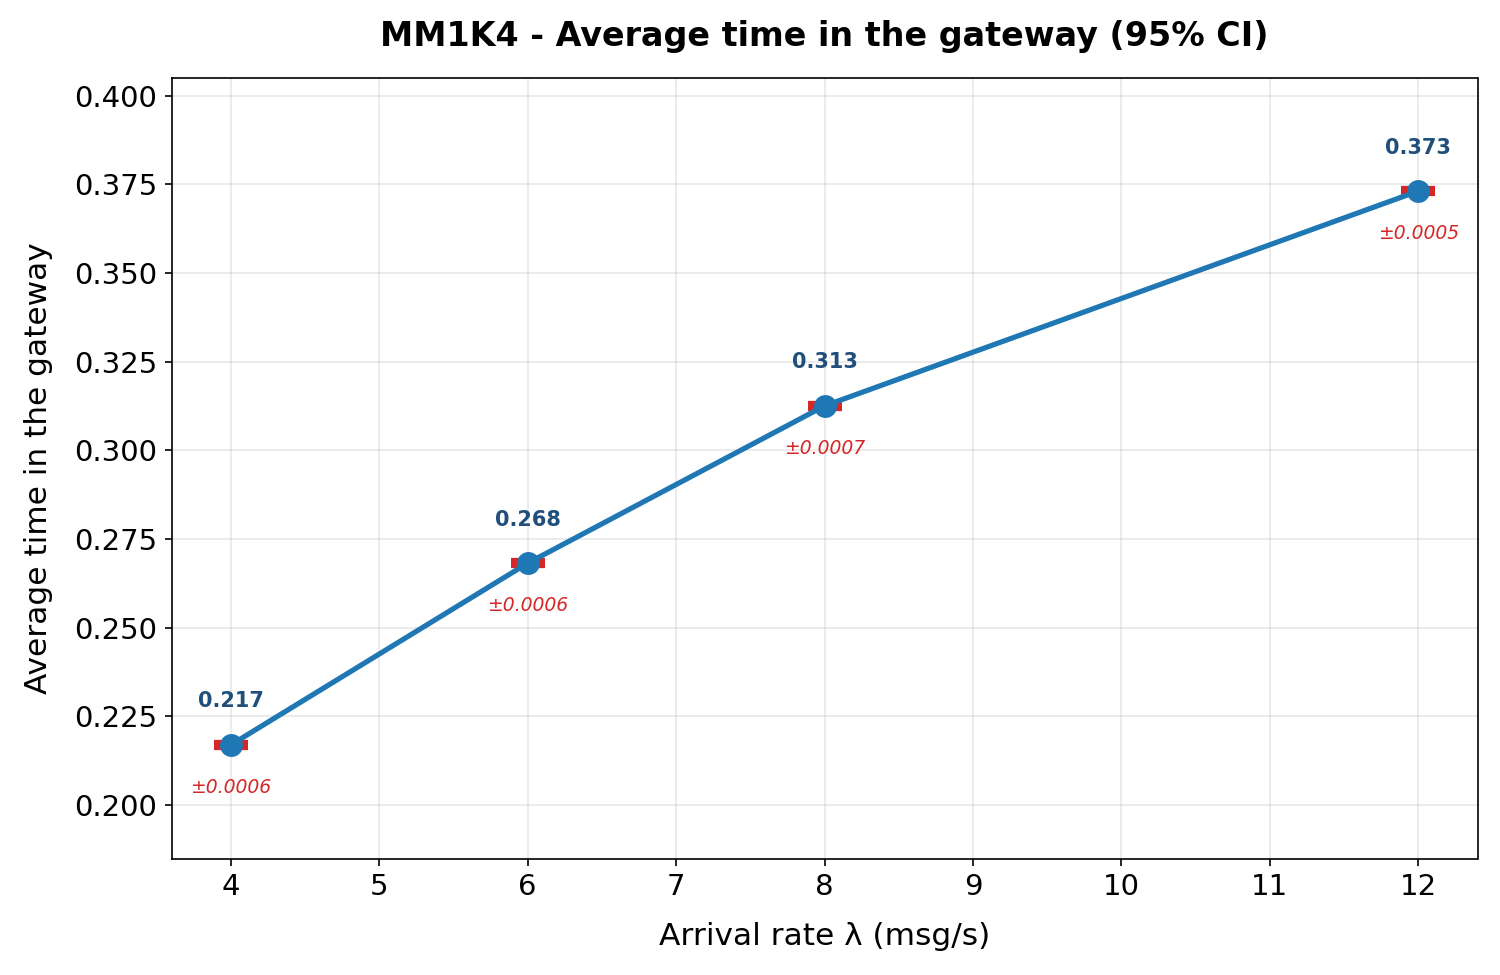
\includegraphics[width=0.75\textwidth]{../outputs/plots/MM1K4-avg_response_time.png}
    \caption{M/M/1/4: Average time in the gateway vs. arrival rate. With 95\% CI error bars.}
    \label{fig:mm1k4-response_time}
\end{figure}

\subsubsection{Average Time in the Servers}

\begin{figure}[H]
    \centering
    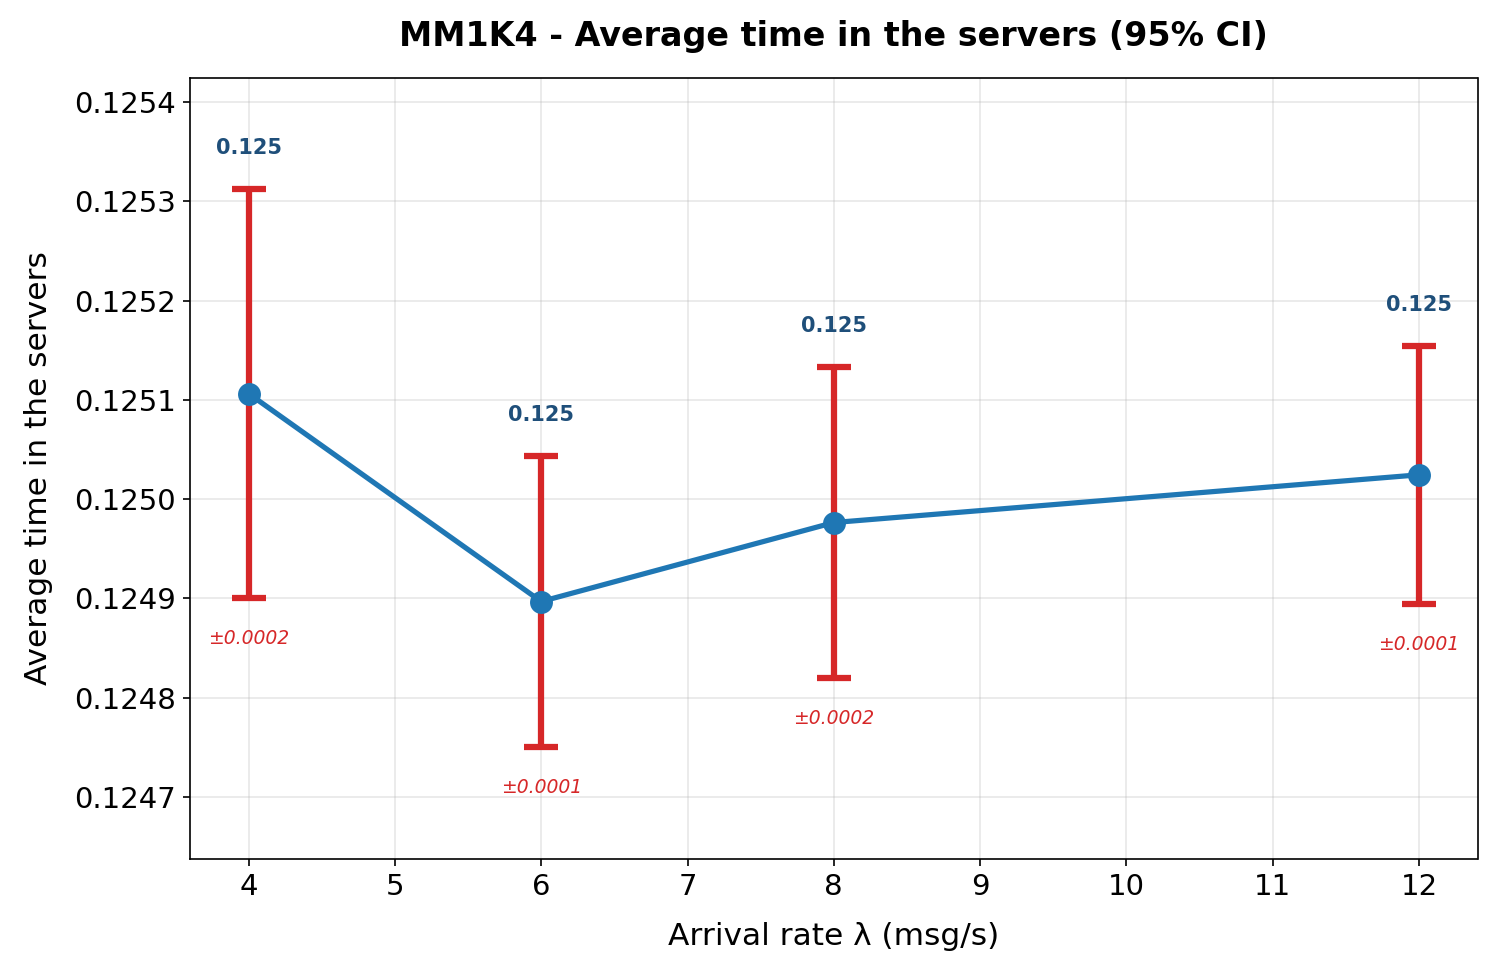
\includegraphics[width=0.75\textwidth]{../outputs/plots/MM1K4-avg_time_in_servers.png}
    \caption{M/M/1/4: Average time in the servers vs. arrival rate. With 95\% CI error bars.}
    \label{fig:mm1k4-time_in_servers}
\end{figure}

\subsubsection{Throughput}

\begin{figure}[H]
    \centering
    
\includegraphics[width=0.75\textwidth]{../outputs/plots/MM1K4-throughput.png}
    \caption{M/M/1/4: Throughput vs. arrival rate. With 95\% CI error bars.}
    \label{fig:mm1k4-throughput}
\end{figure}

\subsubsection{Drop Probability}

\begin{figure}[H]
    \centering
    
\includegraphics[width=0.75\textwidth]{../outputs/plots/MM1K4-drop_probability.png}
    \caption{M/M/1/4: Drop probability vs. arrival rate. With 95\% CI error bars.}
    \label{fig:mm1k4-drop}
\end{figure}

\subsubsection{Observations}

For M/M/1/4 (capacity 4):

\begin{itemize}
    \item \textbf{Low load ($\lambda = 4$):} Capacity is barely a constraint at this load. Drop probability is low ($\sim 3$\%) and metrics are comparable to the unlimited M/M/1 model.

    \item \textbf{Moderate loads ($\lambda = 6, 8$):} Drops become noticeable: $\sim 10\%$ at $\lambda = 6$ and $\sim 20\%$ at $\lambda = 8$. System occupancy is capped by the limit of 4, so throughput no longer tracks the arrival rate.

    \item \textbf{$\lambda = 12$ (high overload):} Drop probability reaches $\sim 0.38$, meaning over a third of arriving requests are turned away. The effective throughput is reduced accordingly.

    \item \textbf{Queue Statistics:} Average queue length is capped by the capacity constraint. The average wait time may be lower than M/M/1 due to fewer arrivals being accepted.

    \item \textbf{Practical Relevance:} This model simulates systems with limited buffers (e.g., network queues, call centers with limited trunk groups). The loss probability is a key metric for service level agreements.
\end{itemize}

\subsection{M/M/1/8: Single Server with Capacity 8}

\subsubsection{Theoretical Background}

This model follows the same M/M/1/K formulation as M/M/1/4, but with capacity $K = 8$ instead of 4. The larger buffer allows more queued messages before blocking occurs:

\begin{itemize}
    \item Loss probability: $P_K = (1-\rho) \rho^K / (1 - \rho^{K+1})$
    \item Effective arrival rate: $\lambda_{\text{eff}} = \lambda(1 - P_K)$
    \item With $\mu = 8$, the server reaches saturation at $\lambda \ge 8$
\end{itemize}

The extra buffer space (4 more slots compared to M/M/1/4) reduces the drop probability at moderate loads, but the system still experiences losses once the buffer is exhausted.

\subsubsection{Average System Occupancy}

\begin{figure}[H]
    \centering
    
\includegraphics[width=0.75\textwidth]{../outputs/plots/MM1K8-avg_n_system.png}
    \caption{M/M/1/8: Average system occupancy vs. arrival rate. With 95\% CI error bars.}
    \label{fig:mm1k8-n_system}
\end{figure}

\subsubsection{Average Messages in Queue}

\begin{figure}[H]
    \centering
    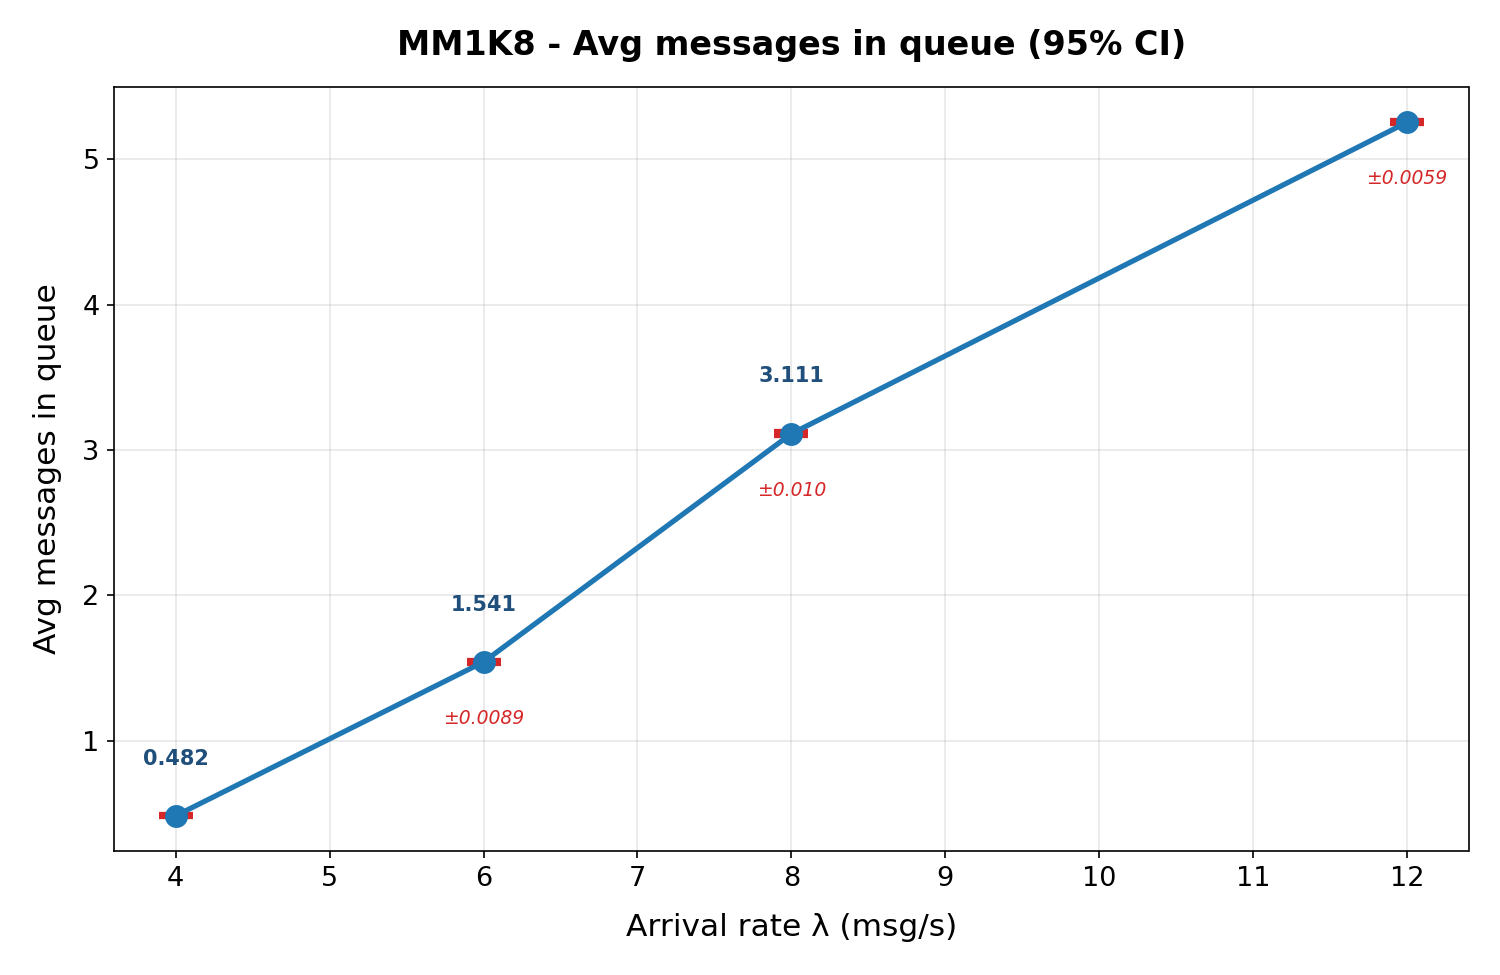
\includegraphics[width=0.75\textwidth]{../outputs/plots/MM1K8-avg_n_queue.png}
    \caption{M/M/1/8: Average number of messages in queue vs. arrival rate. With 95\% CI error bars.}
    \label{fig:mm1k8-n_queue}
\end{figure}

\subsubsection{Average Queue Waiting Time}

\begin{figure}[H]
    \centering
    
\includegraphics[width=0.75\textwidth]{../outputs/plots/MM1K8-avg_wait_queue.png}
    \caption{M/M/1/8: Average queue wait time vs. arrival rate. With 95\% CI error bars.}
    \label{fig:mm1k8-wait_queue}
\end{figure}

\subsubsection{Average Time in the Gateway}

\begin{figure}[H]
    \centering
    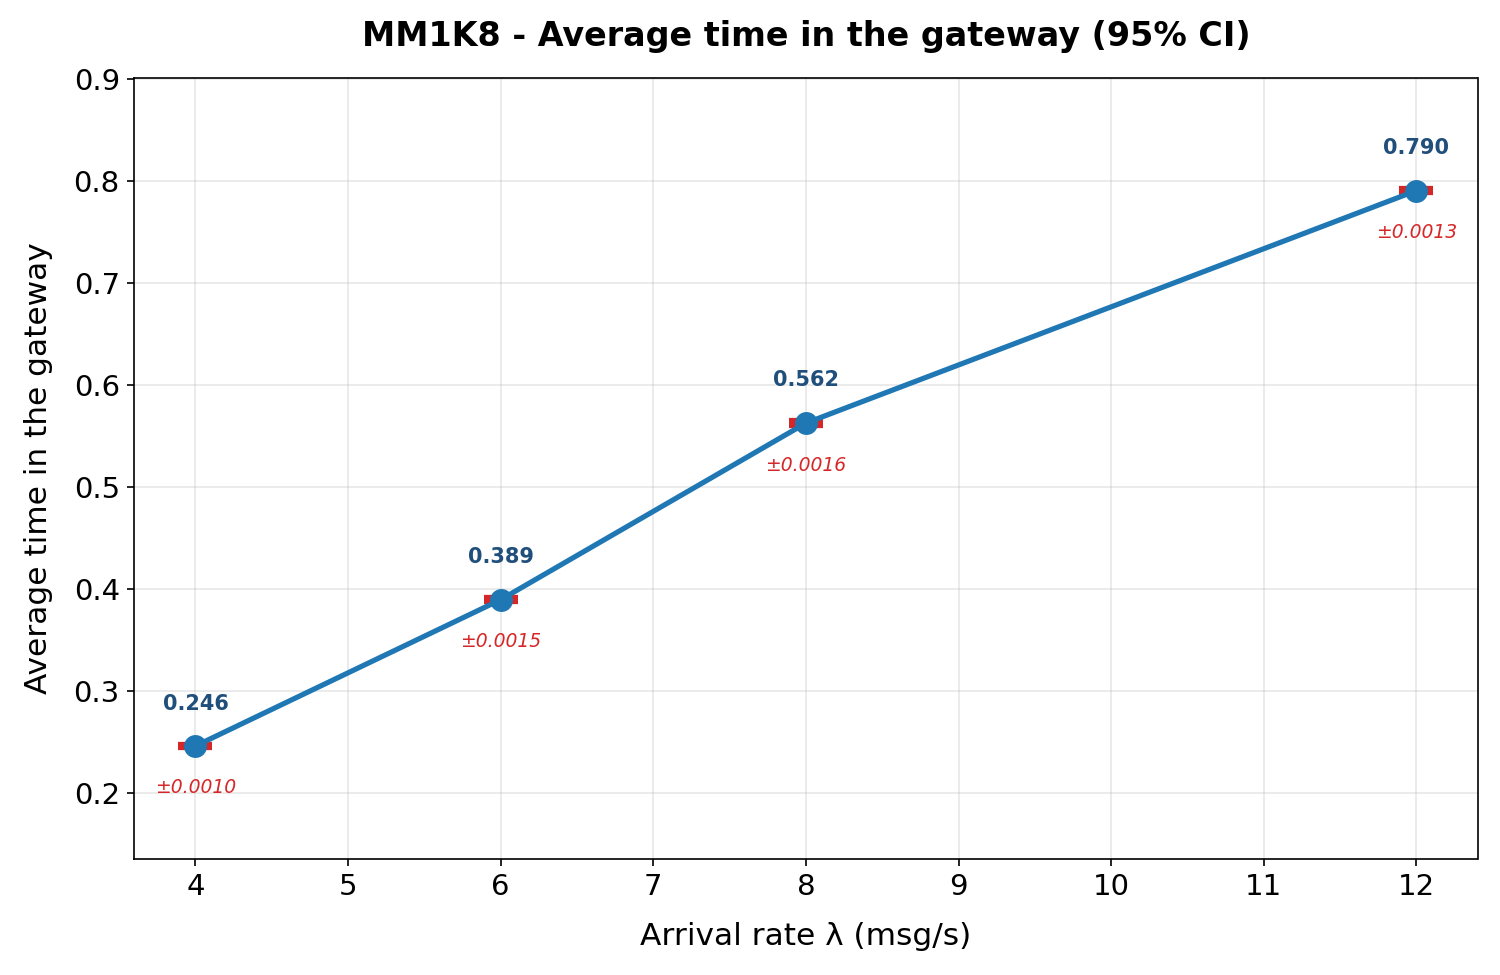
\includegraphics[width=0.75\textwidth]{../outputs/plots/MM1K8-avg_response_time.png}
    \caption{M/M/1/8: Average time in the gateway vs. arrival rate. With 95\% CI error bars.}
    \label{fig:mm1k8-response_time}
\end{figure}

\subsubsection{Average Time in the Servers}

\begin{figure}[H]
    \centering
    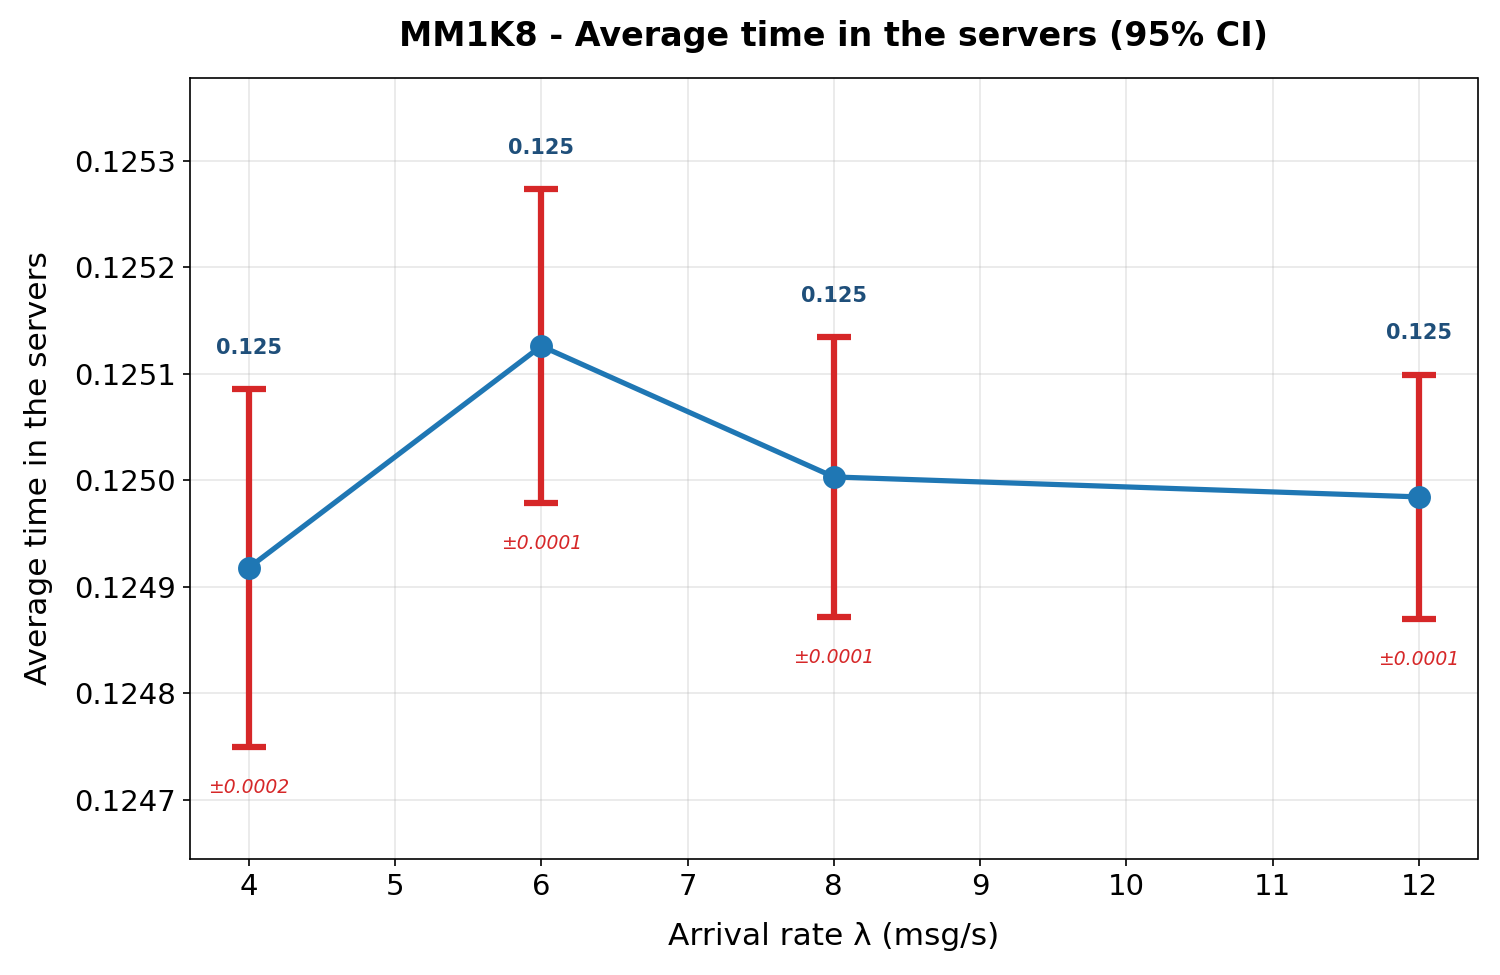
\includegraphics[width=0.75\textwidth]{../outputs/plots/MM1K8-avg_time_in_servers.png}
    \caption{M/M/1/8: Average time in the servers vs. arrival rate. With 95\% CI error bars.}
    \label{fig:mm1k8-time_in_servers}
\end{figure}

\subsubsection{Throughput}

\begin{figure}[H]
    \centering
    
\includegraphics[width=0.75\textwidth]{../outputs/plots/MM1K8-throughput.png}
    \caption{M/M/1/8: Throughput vs. arrival rate. With 95\% CI error bars.}
    \label{fig:mm1k8-throughput}
\end{figure}

\subsubsection{Drop Probability}

\begin{figure}[H]
    \centering
    
\includegraphics[width=0.75\textwidth]{../outputs/plots/MM1K8-drop_probability.png}
    \caption{M/M/1/8: Drop probability vs. arrival rate. With 95\% CI error bars.}
    \label{fig:mm1k8-drop}
\end{figure}

\subsubsection{Observations}

For M/M/1/8 (capacity 8):

\begin{itemize}
    \item \textbf{Intermediate Load:} Compared to M/M/1/4, the larger buffer allows more entities to be queued before losses occur.

    \item \textbf{Transition Region:} At $\lambda = 6$, losses are still negligible; by $\lambda = 12$, drops are significant but perhaps less severe than M/M/1/4 due to the extra buffer space.

    \item \textbf{Utilization Trade-off:} Larger buffers improve the throughput and reduce drop probability, but they also increase the average queue wait time for those arrivals that do enter the system.

    \item \textbf{Capacity Effect:} The doubling of capacity from K=4 to K=8 reduces losses, particularly at moderate to high loads. This illustrates the buffer-size trade-off in network design.
\end{itemize}

\subsection{M/M/3/8: Three Parallel Servers with Capacity 8}

\subsubsection{Theoretical Background}

M/M/c/K models allow $c$ parallel servers, each with service rate $\mu$. The aggregate service capacity is $c \times \mu$. With $c = 3$ and $\mu = 8$, the total service rate is 24 messages/s.

Key differences from single-server models:
\begin{itemize}
    \item When $c$ entities are in service, the next arrival joins the queue (not the server)
    \item System is stable if $\lambda < c \times \mu$ (in our case, stable for all tested $\lambda$ since $12 < 24$)
    \item Losses still occur if capacity $K$ is exceeded (we have $K = 8$)
\end{itemize}

\subsubsection{Average System Occupancy}

\begin{figure}[H]
    \centering
    
\includegraphics[width=0.75\textwidth]{../outputs/plots/MM3K8-avg_n_system.png}
    \caption{M/M/3/8: Average system occupancy vs. arrival rate. With 95\% CI error bars.}
    \label{fig:mm3k8-n_system}
\end{figure}

\subsubsection{Average Messages in Queue}

\begin{figure}[H]
    \centering
    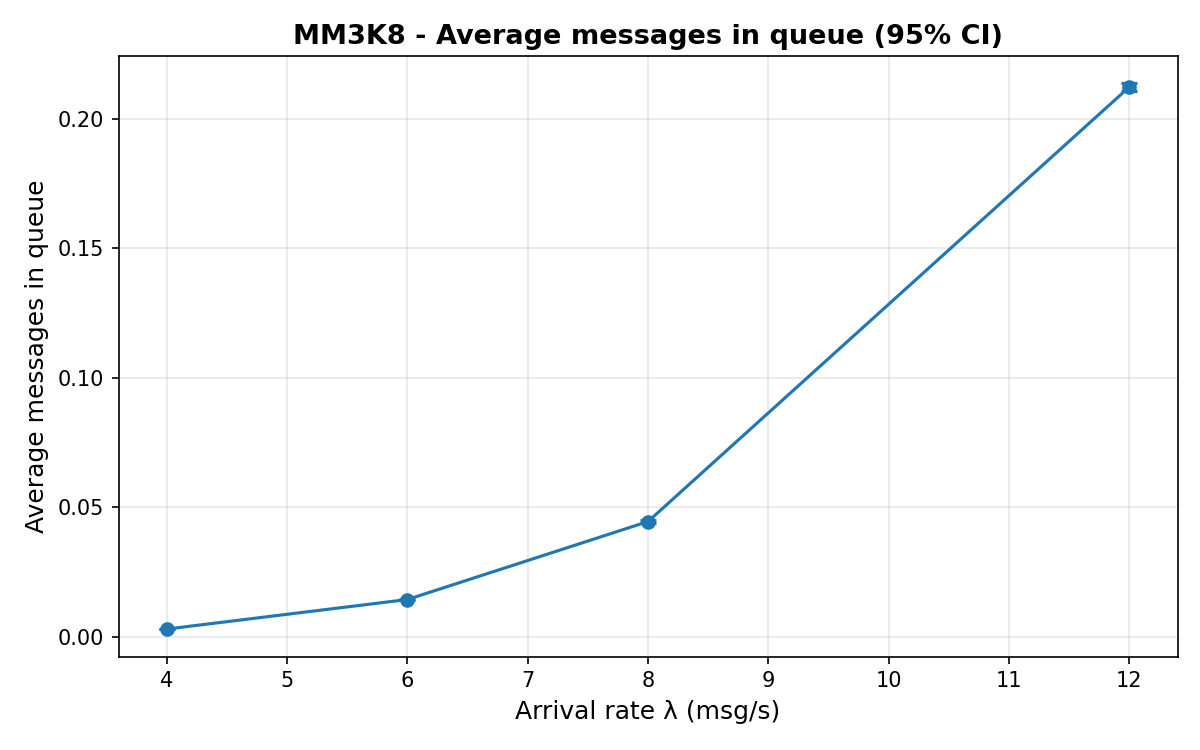
\includegraphics[width=0.75\textwidth]{../outputs/plots/MM3K8-avg_n_queue.png}
    \caption{M/M/3/8: Average number of messages in queue vs. arrival rate. With 95\% CI error bars.}
    \label{fig:mm3k8-n_queue}
\end{figure}

\subsubsection{Average Queue Waiting Time}

\begin{figure}[H]
    \centering
    
\includegraphics[width=0.75\textwidth]{../outputs/plots/MM3K8-avg_wait_queue.png}
    \caption{M/M/3/8: Average queue wait time vs. arrival rate. With 95\% CI error bars.}
    \label{fig:mm3k8-wait_queue}
\end{figure}

\subsubsection{Average Time in the Gateway}

\begin{figure}[H]
    \centering
    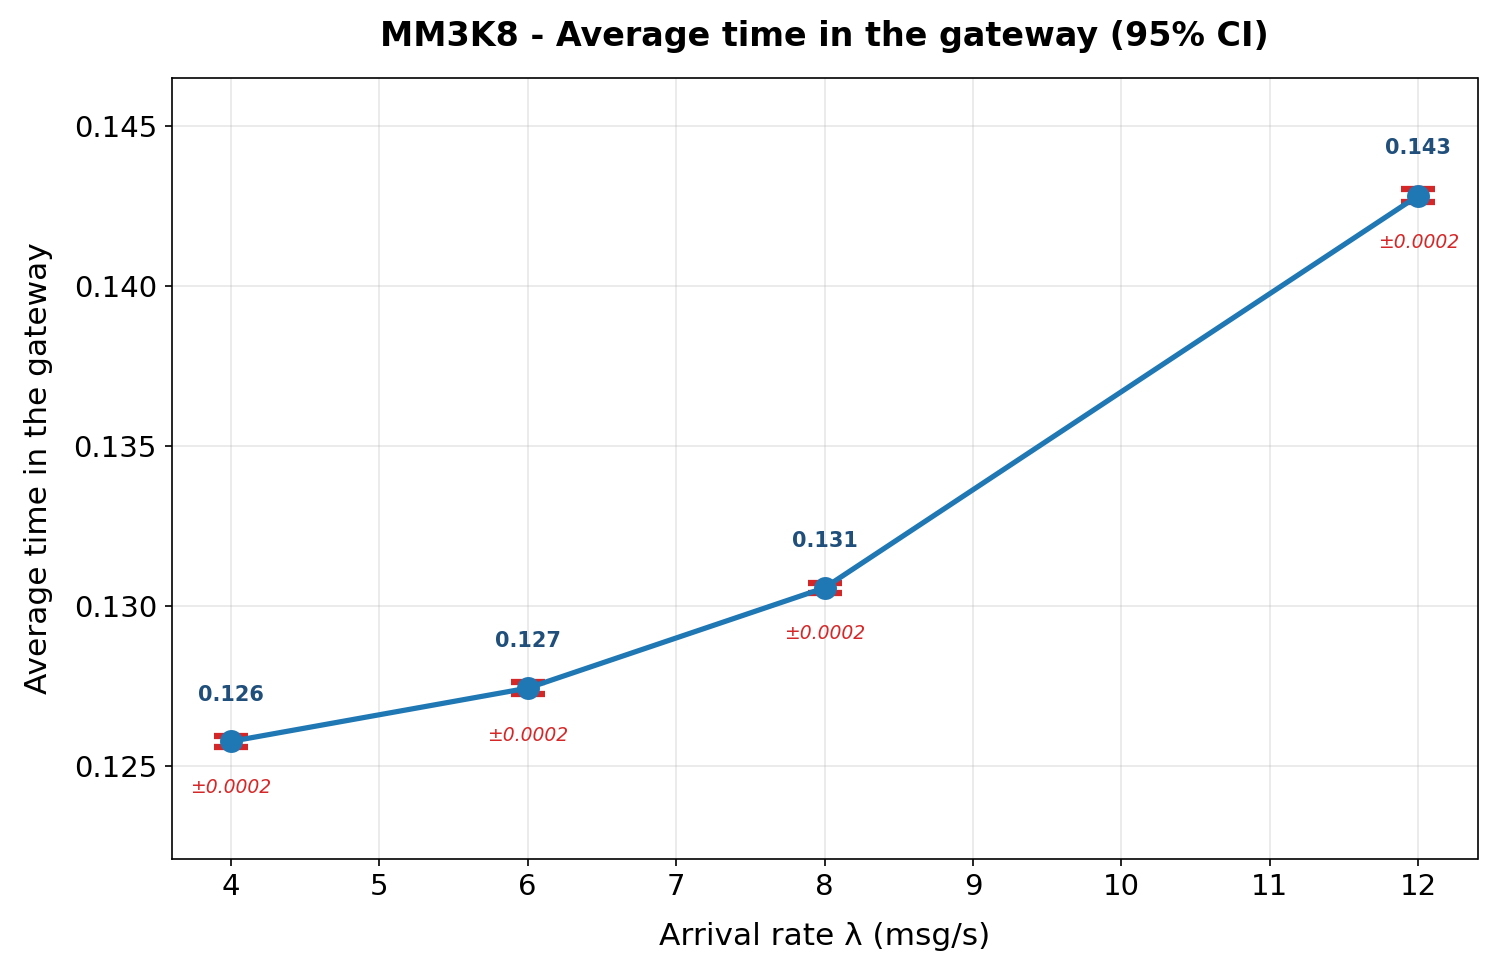
\includegraphics[width=0.75\textwidth]{../outputs/plots/MM3K8-avg_response_time.png}
    \caption{M/M/3/8: Average time in the gateway vs. arrival rate. With 95\% CI error bars.}
    \label{fig:mm3k8-response_time}
\end{figure}

\subsubsection{Average Time in the Servers}

\begin{figure}[H]
    \centering
    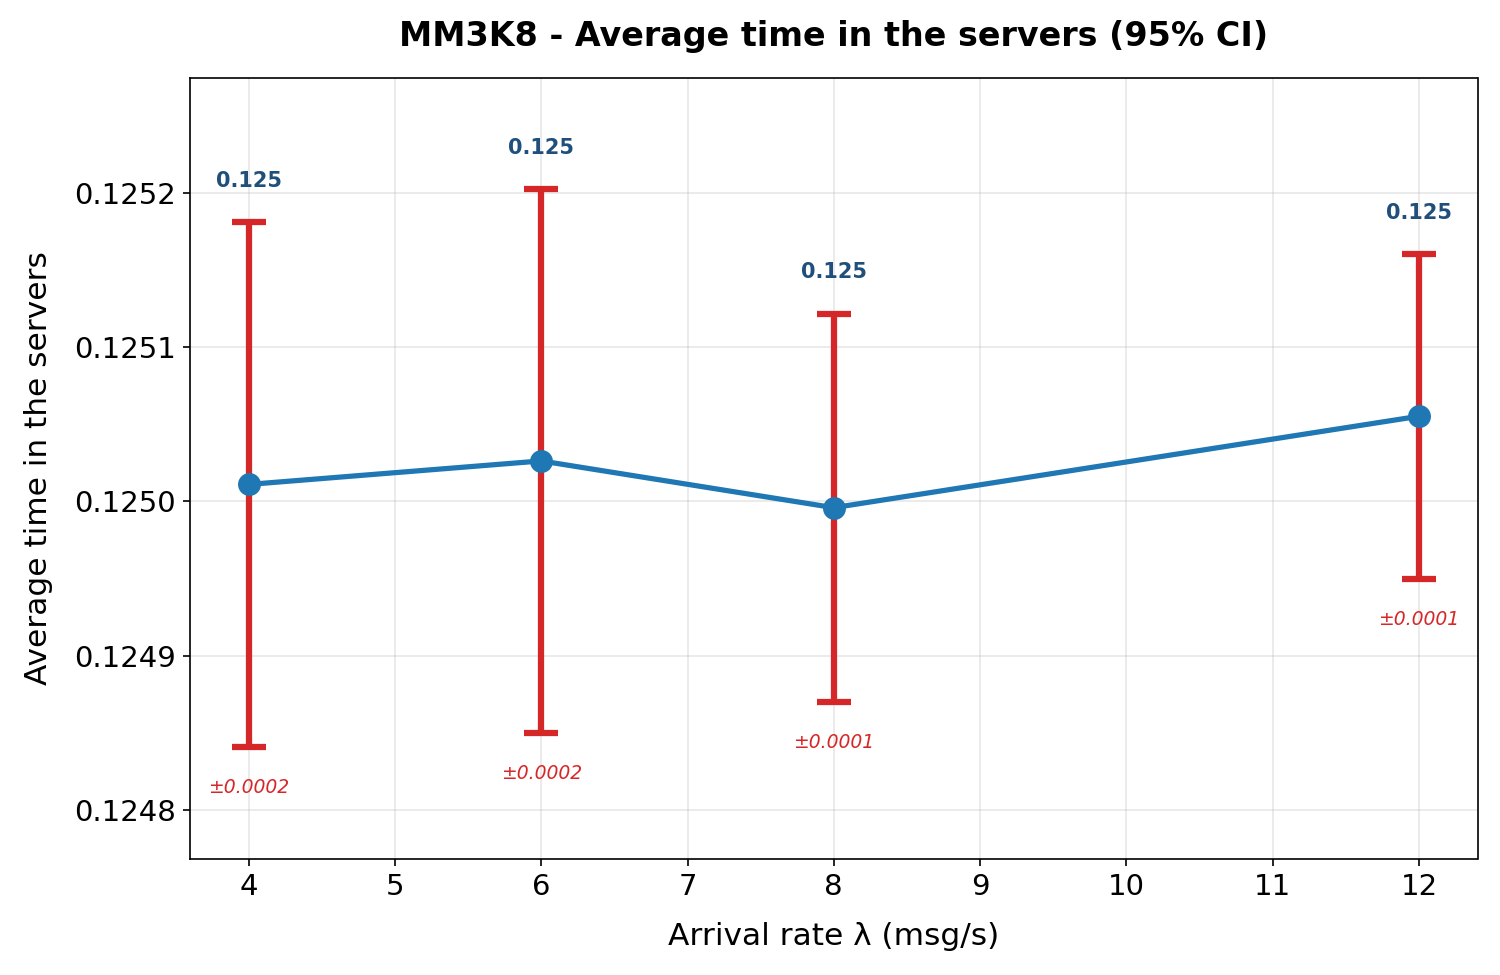
\includegraphics[width=0.75\textwidth]{../outputs/plots/MM3K8-avg_time_in_servers.png}
    \caption{M/M/3/8: Average time in the servers vs. arrival rate. With 95\% CI error bars.}
    \label{fig:mm3k8-time_in_servers}
\end{figure}

\subsubsection{Throughput}

\begin{figure}[H]
    \centering
    
\includegraphics[width=0.75\textwidth]{../outputs/plots/MM3K8-throughput.png}
    \caption{M/M/3/8: Throughput vs. arrival rate. With 95\% CI error bars.}
    \label{fig:mm3k8-throughput}
\end{figure}

\subsubsection{Drop Probability}

\begin{figure}[H]
    \centering
    
\includegraphics[width=0.75\textwidth]{../outputs/plots/MM3K8-drop_probability.png}
    \caption{M/M/3/8: Drop probability vs. arrival rate. With 95\% CI error bars.}
    \label{fig:mm3k8-drop}
\end{figure}

\subsubsection{Observations}

For M/M/3/8 (three servers, capacity 8):

\begin{itemize}
    \item \textbf{Aggregate Capacity:} With three parallel servers, the system can handle up to 24 messages/s. Thus, all tested arrival rates ($\lambda \le 12$) are well below saturation.

    \item \textbf{Reduced Congestion:} Compared to single-server models, the M/M/3 system experiences significantly lower queue waits and occupancy. At $\lambda = 12$, some entities are in the queue, but the waiting time is very short.

    \item \textbf{Low Loss Rates:} Drop probability is near zero for all tested loads because the large aggregate service capacity (24 vs. max arrival 12) ensures most arrivals are accepted and served quickly.

    \item \textbf{Scalability:} This model demonstrates the benefit of parallelism. By adding servers, the system can handle higher load while maintaining acceptable delays and low loss rates.

    \item \textbf{Practical Example:} This represents a web server cluster with 3 backend servers or a call center with 3 agents handling the same type of request.
\end{itemize}

\section{Comparative Analysis}

\subsection{Impact of Capacity}

\begin{table}[H]
    \centering
    \begin{tabular}{lcccc}
        \toprule
        \textbf{Model} & \textbf{Servers} & \textbf{Capacity} & \textbf{Max Service} & \textbf{Stability} \\
        \midrule
        M/M/1          & 1                & $\infty$          & 8 msg/s              & $\lambda < 8$      \\
        M/M/1/4        & 1                & 4                 & 8 msg/s              & Limited buffer     \\
        M/M/1/8        & 1                & 8                 & 8 msg/s              & Limited buffer     \\
        M/M/3/8        & 3                & 8                 & 24 msg/s             & $\lambda < 24$     \\
        \bottomrule
    \end{tabular}
    \caption{Queueing model comparison.}
    \label{tab:model-comparison}
\end{table}

Key observations:

\begin{enumerate}
    \item \textbf{Single vs. Multiple Servers:} M/M/3/8 with three servers provides dramatically better performance than M/M/1/8 (single server) despite the same capacity limit of 8. The aggregate service rate is 3 times higher, enabling the system to absorb higher loads.

    \item \textbf{Capacity Limits:} Finite-capacity models (M/M/1/4, M/M/1/8) incur losses under load, reducing effective throughput. M/M/1 with unlimited capacity can theoretically handle any load (though queue grows unbounded if $\lambda \ge \mu$).

    \item \textbf{Trade-offs:}
          \begin{itemize}
              \item Larger capacity (M/M/1/8 vs. M/M/1/4): Better throughput and lower loss, but customers may wait longer in a larger queue.
              \item More servers (M/M/3/8 vs. M/M/1/8): Lower delays, better throughput, requires more investment.
          \end{itemize}
\end{enumerate}

\subsection{Load Dependency}

All metrics depend strongly on the arrival rate:

\begin{itemize}
    \item \textbf{Low Load ($\lambda = 4$):} All models behave similarly; capacity and parallelism constraints are not active. Queue waits are minimal.

    \item \textbf{Moderate Load ($\lambda = 6, 8$):} Differences emerge. Finite-capacity systems begin to lose packets. Multi-server systems show advantage over single-server.

    \item \textbf{High Load ($\lambda = 12$):} Differences are most pronounced. Single-server systems approach saturation or stability limits; multi-server systems remain stable with low delays.

    \item \textbf{Confidence Intervals:} Higher load generally correlates with larger CI widths, indicating more variability in transient behavior.
\end{itemize}

\section{Implementation Validation}

\subsection{Class-Level Unit Tests}

All classes pass the assigned unit tests:

\begin{itemize}
    \item \texttt{test\_message()}: Message creation, ID assignment, source/destination fields
    \item \texttt{test\_event()}: Event creation with type, timestamp, message reference
    \item \texttt{test\_scheduler()}: Chronological ordering, heap-based insertion, event popping in correct order
    \item \texttt{test\_client()}: Exponential inter-arrival generation, message creation
    \item \texttt{test\_queue()}: FIFO push/pop, capacity tracking
    \item \texttt{test\_server()}: Service initiation, completion, busy/idle state
    \item \texttt{test\_gateway()}: Queue + server orchestration, RECV/DEPT handling, admission control
\end{itemize}

\subsection{Trace Validation}

Sample event traces were generated and manually inspected to confirm:

\begin{enumerate}
    \item Events are in chronological order (strictly increasing timestamps)
    \item Event types match expected flow (SEND $\to$ RECV $\to$ DEPT)
    \item Message IDs are consistent across events
    \item Source and destination fields are correctly propagated
    \item 1-second propagation delay is correctly applied between SEND and RECV
\end{enumerate}

\subsection{Metrics Sanity Checks}

Generated metrics were validated against queueing theory predictions and intuition:

\begin{enumerate}
    \item \textbf{Stability Check:} For $\lambda < \mu$, average occupancy and queue wait are finite and reasonable.

    \item \textbf{Throughput Check:} Measured throughput never exceeds service capacity $\mu \times \text{servers}$ or effective capacity due to losses.

    \item \textbf{Load Dependency:} As expected, metrics increase as the arrival rate goes up.

    \item \textbf{Server Utilization:} Matches the theoretical value. For example, at $\lambda = 6, \mu = 8$:
          \begin{equation}
              \rho_{\text{theory}} = \frac{6}{8} = 0.75
          \end{equation}
          Our simulation gives $\rho_{\text{sim}} \approx 0.75$, which confirms correctness.

    \item \textbf{Multi-Server Advantage:} M/M/3/8 consistently outperforms M/M/1/8 (lower delays, higher throughput, zero losses) due to parallel service.
\end{enumerate}

\section{Conclusion}

In this lab, we built and used a discrete-event simulator to evaluate the performance of four queueing models under varying load.

\subsection{Key Findings}

\begin{enumerate}
    \item \textbf{Model Behavior:} All four models behave as expected from queueing theory. Metrics respond to load changes, capacity constraints, and the number of servers as predicted.

    \item \textbf{Impact of Parallelism:} Adding more servers (M/M/3 vs. M/M/1) improves performance significantly, allowing the system to handle higher loads with lower latency.

    \item \textbf{Capacity Trade-offs:} Finite-capacity systems prevent buffer overflow but drop messages under high load. Larger buffers (K=8 vs. K=4) reduce drops but increase queue wait times.

    \item \textbf{Stability:} The M/M/1 model with $\lambda \ge \mu$ is unstable and the queue keeps growing during the simulation. Adding a finite buffer prevents unbounded growth but causes losses.

    \item \textbf{Confidence Intervals:} We report all metrics with 95\% CI. The intervals are wider at higher loads, which reflects the increased randomness under stress.

    \item \textbf{Implementation:} The object-oriented design made it straightforward to separate concerns and test each component individually.
\end{enumerate}

\subsection{Practical Implications}

\begin{enumerate}
    \item \textbf{Capacity Planning:} This kind of simulation could help estimate how many servers and how much buffer space are needed to meet target loss rates and response times.

    \item \textbf{Load Balancing:} The results show that distributing traffic across multiple servers improves performance, which is why load balancing is important in real systems.

    \item \textbf{Admission Control:} When the system is overloaded, some mechanism for rejecting requests (like the finite buffer does) prevents complete breakdown.

    \item \textbf{Peak Load:} The M/M/1 results at $\lambda = 12$ show what happens during traffic spikes. Systems need some form of protection when arrival rates exceed service capacity.
\end{enumerate}

\section{Reproducibility}

All code, configuration, and generated outputs are stored in the GitHub repository:

\begin{center}
    \url{https://github.com/abdulhadihub/cnam-performance-evaluation-course/tree/main/lab-2}
\end{center}

To reproduce results:

\begin{enumerate}
    \item Clone the repository
    \item Install dependencies: \texttt{uv sync}
    \item Run experiments: \texttt{uv run python main.py experiments --replications 100 --sim-time 5000}
    \item Inspect outputs in \texttt{outputs/results/} and \texttt{outputs/plots/}
\end{enumerate}

All runs use deterministic seeding, ensuring identical results across different systems and time periods.

\end{document}
